%!TEX root = main.tex


Fingerprints are ridge and valley patterns present on the surface of human fingertips.
%
Fingerprint matching has played a critical role in identifying suspects and criminals.
%
Due to fingerprint’s high discriminability and persistence over time, fingerprint-based person recognition systems have been widely deployed.
%
Fingerprint recognition systems have played a crucial role in various applications, including law enforcement, forensics, physical and logical access control, border crossing and civil registry.
%
Fingerprint features can be divided into three major categories based on the granularity at which they are extracted: level 1, level 2 and level 3 features.
%
In this project, we are going to implment a fingerprint recognition system that classify a fingerprin into the following 5 categories:
%
A=Arch, L=Left Loop, R=Right Loop, T=Tented Arch, W=Whorl.
%
As shown in Fig.\ref{fig.fingerprint_classes}

\begin{figure}[!ht]
	\begin{center}
		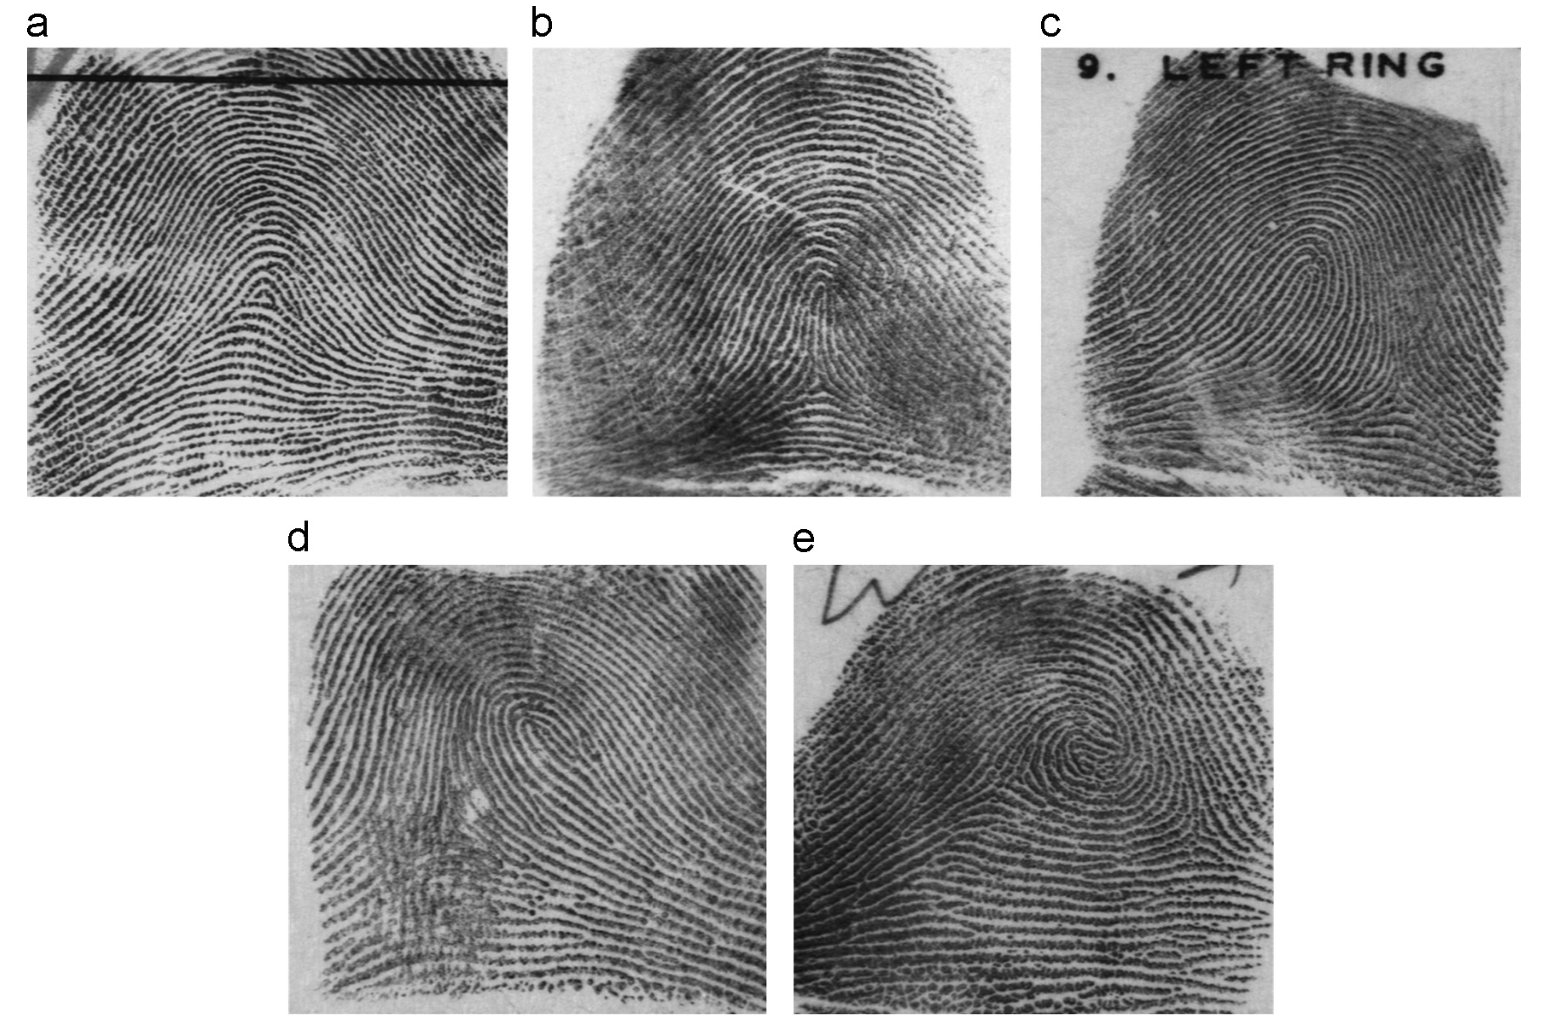
\includegraphics[width=8cm]{fig/Fingerprint_classes.png}
	\end{center}
	\caption{Fingerprint classes: Top row: arch, left loop, and right loop. Bottom row: tented arch, whorl, and twin-loop. Triangles mark deltas; diamonds mark cores and whorls. Note that there is an invisible delta further to the bottom left of the last image, which actually shows a tented-arch-and-loop rather than a twin-loop. These are based on images from the FVC 2000, Database 2a [34]. }
	\label{fig.fingerprint_classes}
\end{figure}

From the last image in Fig.\ref{fig.fingerprint_classes} we can see that one fingerprint may be classified into multiple categories at the same time.